\documentclass{article}

\usepackage{minitoc}
\usepackage{tabularx}
\usepackage{booktabs}
\usepackage{graphicx}
\usepackage{hyperref}
\usepackage{xcolor}
\usepackage{blkarray}
\usepackage{amsthm, amssymb, amsmath}
\usepackage{caption}
\usepackage{subcaption}
\usepackage{multirow}
\usepackage[ruled,vlined]{algorithm2e}

\usepackage{natbib}
\bibliographystyle{abbrvnat}

\theoremstyle{definition}
\newtheorem{definition}{Definition}[section]
\newtheorem{theorem}{Theorem}[section]
\newtheorem{lemma}[theorem]{Lemma}
\newtheorem{conjecture}[theorem]{Conjecture}

\usepackage[margin=2.5cm, includefoot, footskip=30pt]{geometry}
\pagestyle{plain}
\setlength{\parindent}{0em}
\setlength{\parskip}{1em}

\renewcommand{\baselinestretch}{1}

\usepackage{standalone}

\newtheorem{proposition}{Proposition}

\title{$n-$bits reactive strategies}

\author{Nikoleta E. Glynatsi, Ethan Akin, Martin Nowak, Christian Hilbe}
\date{}

\begin{document}

\maketitle

The donation game is a two person symmetric game that provides a simple model of
cooperation. Each of the two players, simultaneously and independently decide to
cooperate ($C$) or to defect ($D$). A player who cooperates pays a cost \(c >
0\) to provide a benefit \(b > c\) for the co-player. A cooperator either gets
\(b\!-\!c\) (if the co-player also cooperates) or \(-c\) (if the co-player
defects). Respectively, a defector either gets \(b\) (if the co-player
cooperates) or 0 (if the co-player defects), and so, the payoffs of player \(1\)
and \(1\), take the forms $\mathbf{S}_{1} = (b - c, -c, b, 0)$ and
$\mathbf{S}_{2} = (b - c, b, -c, 0)$.

In the iterated version of the game, the two players are required to play an
infinite number of rounds. In repeated games, players can use strategies that
depend on the outcome of the previous rounds. We assume in the following, that the players' decisions only depend on the
outcome of the previous $n$ rounds. To this end, an {\it $n$-history for player
$i \in \{1, 2\}$} is a string $h^i=(a^i_{-n},\ldots,a^i_{-1})\!\in\!\{C,D\}^n$. An entry
$a^i_{-k}$ corresponds to player $i$'s action $k$ rounds ago. Let $H^i$ denote
the space of all $n$-histories for $i \in \{1, 2\}$. Set $H^i$
contains $|H^i|=2^{n}$ elements. A pair $h\!=\!(h^1,h^2)$ is called an {\it
$n$-history of the game}. We use $H=H^1\times H^2$ to denote the space of all
such histories. This set contains $|H|=2^{2n}$ elements.

A subset of these strategies are those that only depend on the
previous round. These are called memory-one strategies. They have been studied
extensively in the literature. Previous work has characterized all memory-one
strategies that are Nash and parters. pattern strategies are a subset of Nash
which ensure that the players share the rewards fairly. Set of strategies as
well that from evolutionary process. Considering strategies that use more
memory can beneficial, as they allow for more coopeartion to evolve, and
as shown in the work of longer memory strategies can be more robust to errors
and in multiagent interactions can be shown to be better as they can exploit
weaker strategies. Exploring analytically or even numerically is an untractable
problem. There are 10. only pure memory-two strategies and 10 memory-three.

Previous work has explored the space of memory-n, n=2 and n-3, space but only
particially, and not the intire space. In this work we exmplore the space
of higher memory strategies. We use a specific s  et of strategies called reactive
thta habe been explored. Reactive strategies are strategies that only depend on
the coplayer's actions. 


In this work we characterise all partner strategies
for reactive-two and reactive-three. We show that when players use reactive
strategies then it is sufficient to check only against self reactive strategies.
For higher n we characterise.

\section{Model}

In this work we explore \textit{reactive strategies} in the infinitely repeated
prisoner's dilemma. The prisoner's dilemma is a two person symmetric game that
provides a simple model of cooperation. Each of the two players, \(p\) and
\(q\), simultaneously and independently decide to cooperate (\(C\)) or to defect
(\(D\)). A player who cooperates pays a cost \(c > 0\) to provide a benefit \(b
> c\) for the co-player. A cooperator either gets \(b\!-\!c\) (if the co-player
also cooperates) or \(-c\) (if the co-player defects). Respectively, a defector
either gets \(b\) (if the co-player cooperates) or 0 (if the co-player defects),
and so, the payoffs of player \(p\) take the form,

\begin{equation}\label{eq:donation_payoffs}
  \begin{blockarray}{ccc}
      & \text{cooperate} & \text{defect} \\
      \begin{block}{c(cc)}
          \text{cooperate} & b\!-\!c & -c \\
          \text{defect} & b & 0 \\
      \end{block}
  \end{blockarray}
\end{equation}

The transpose of (\ref{eq:donation_payoffs}) gives the payoffs of co-player
\(q\). We can also define each player's payoffs as vectors,

\begin{equation}\label{eq:vector_payoffs}
  \mathbf{S}_{p} = (b\!-\!c, -c, b, 0) \quad \textrm{and} \quad  \mathbf{S}_{q} = (b\!-\!c, b, -c, 0).
\end{equation}

We denote the long-term payoffs of players \(p\) and \(q\) as \(\mathbf{s}_{p}\)
and \(\mathbf{s}_{q}\).

\section{Model}

At each round \(t\) of the repeated game, players \(p\) and \(q\) decide on an
action \(a^{p}_{t},\) and \(a^{q}_{t} \in \{C, D\}\) respectively (\textbf{Fig.
1a}). We assume that the players' decisions only depend on the outcome of the
previous \(n\) rounds. An {\it $n$-history for player $p$} is a string
$h^p=(a^p_{-1},\ldots,a^p_{-n})\!\in\!\{C,D\}^n$. Here, an entry $a^p_{-k}$
corresponds to player $p$'s action $k$ rounds ago. Let $H^p$ denote the space of
all $n$-histories of player~$p$. Analogously, we define $H^q$ as the set of
$n$-histories $h^q$ of player~$q$. Sets $H^p$ and $H^q$ contain
$|H^p|=|H^q|=2^{n}$ elements each. A pair $h\!=\!(h^p,h^q)$ is called an {\it
$n$-history of the game}. We use $H=H^p\times H^q$ to denote the space of all
such histories. This set contains $|H|=2^{2n}$ elements.

A {\it memory-$n$} strategy is a vector $\mathbf{p}=(p_h)_{h\in
H}\in[0,1]^{2n}$. Each entry $p_h$ corresponds to the player's cooperation
probability in the next round, depending on the outcome of the previous $n$
rounds.

On the other hand, an {\it $n-$ bit reactive strategy} is a vector
$\mathbf{\hat{p}}=(\hat{p}_h)_{h\in H^q}\in[0,1]^{2n}$. Each entry $\hat{p}_h$
corresponds to the player's cooperation probability in the next round,
depending on the co-player's action(s) of the previous \(n\) rounds. Thus,
\(n\)-bit reactive strategies only depend on the co-player's \(n\)-history
(independent of the focal player's own actions during the past \(n\) rounds).

\begin{figure}[h!]
    \centering
    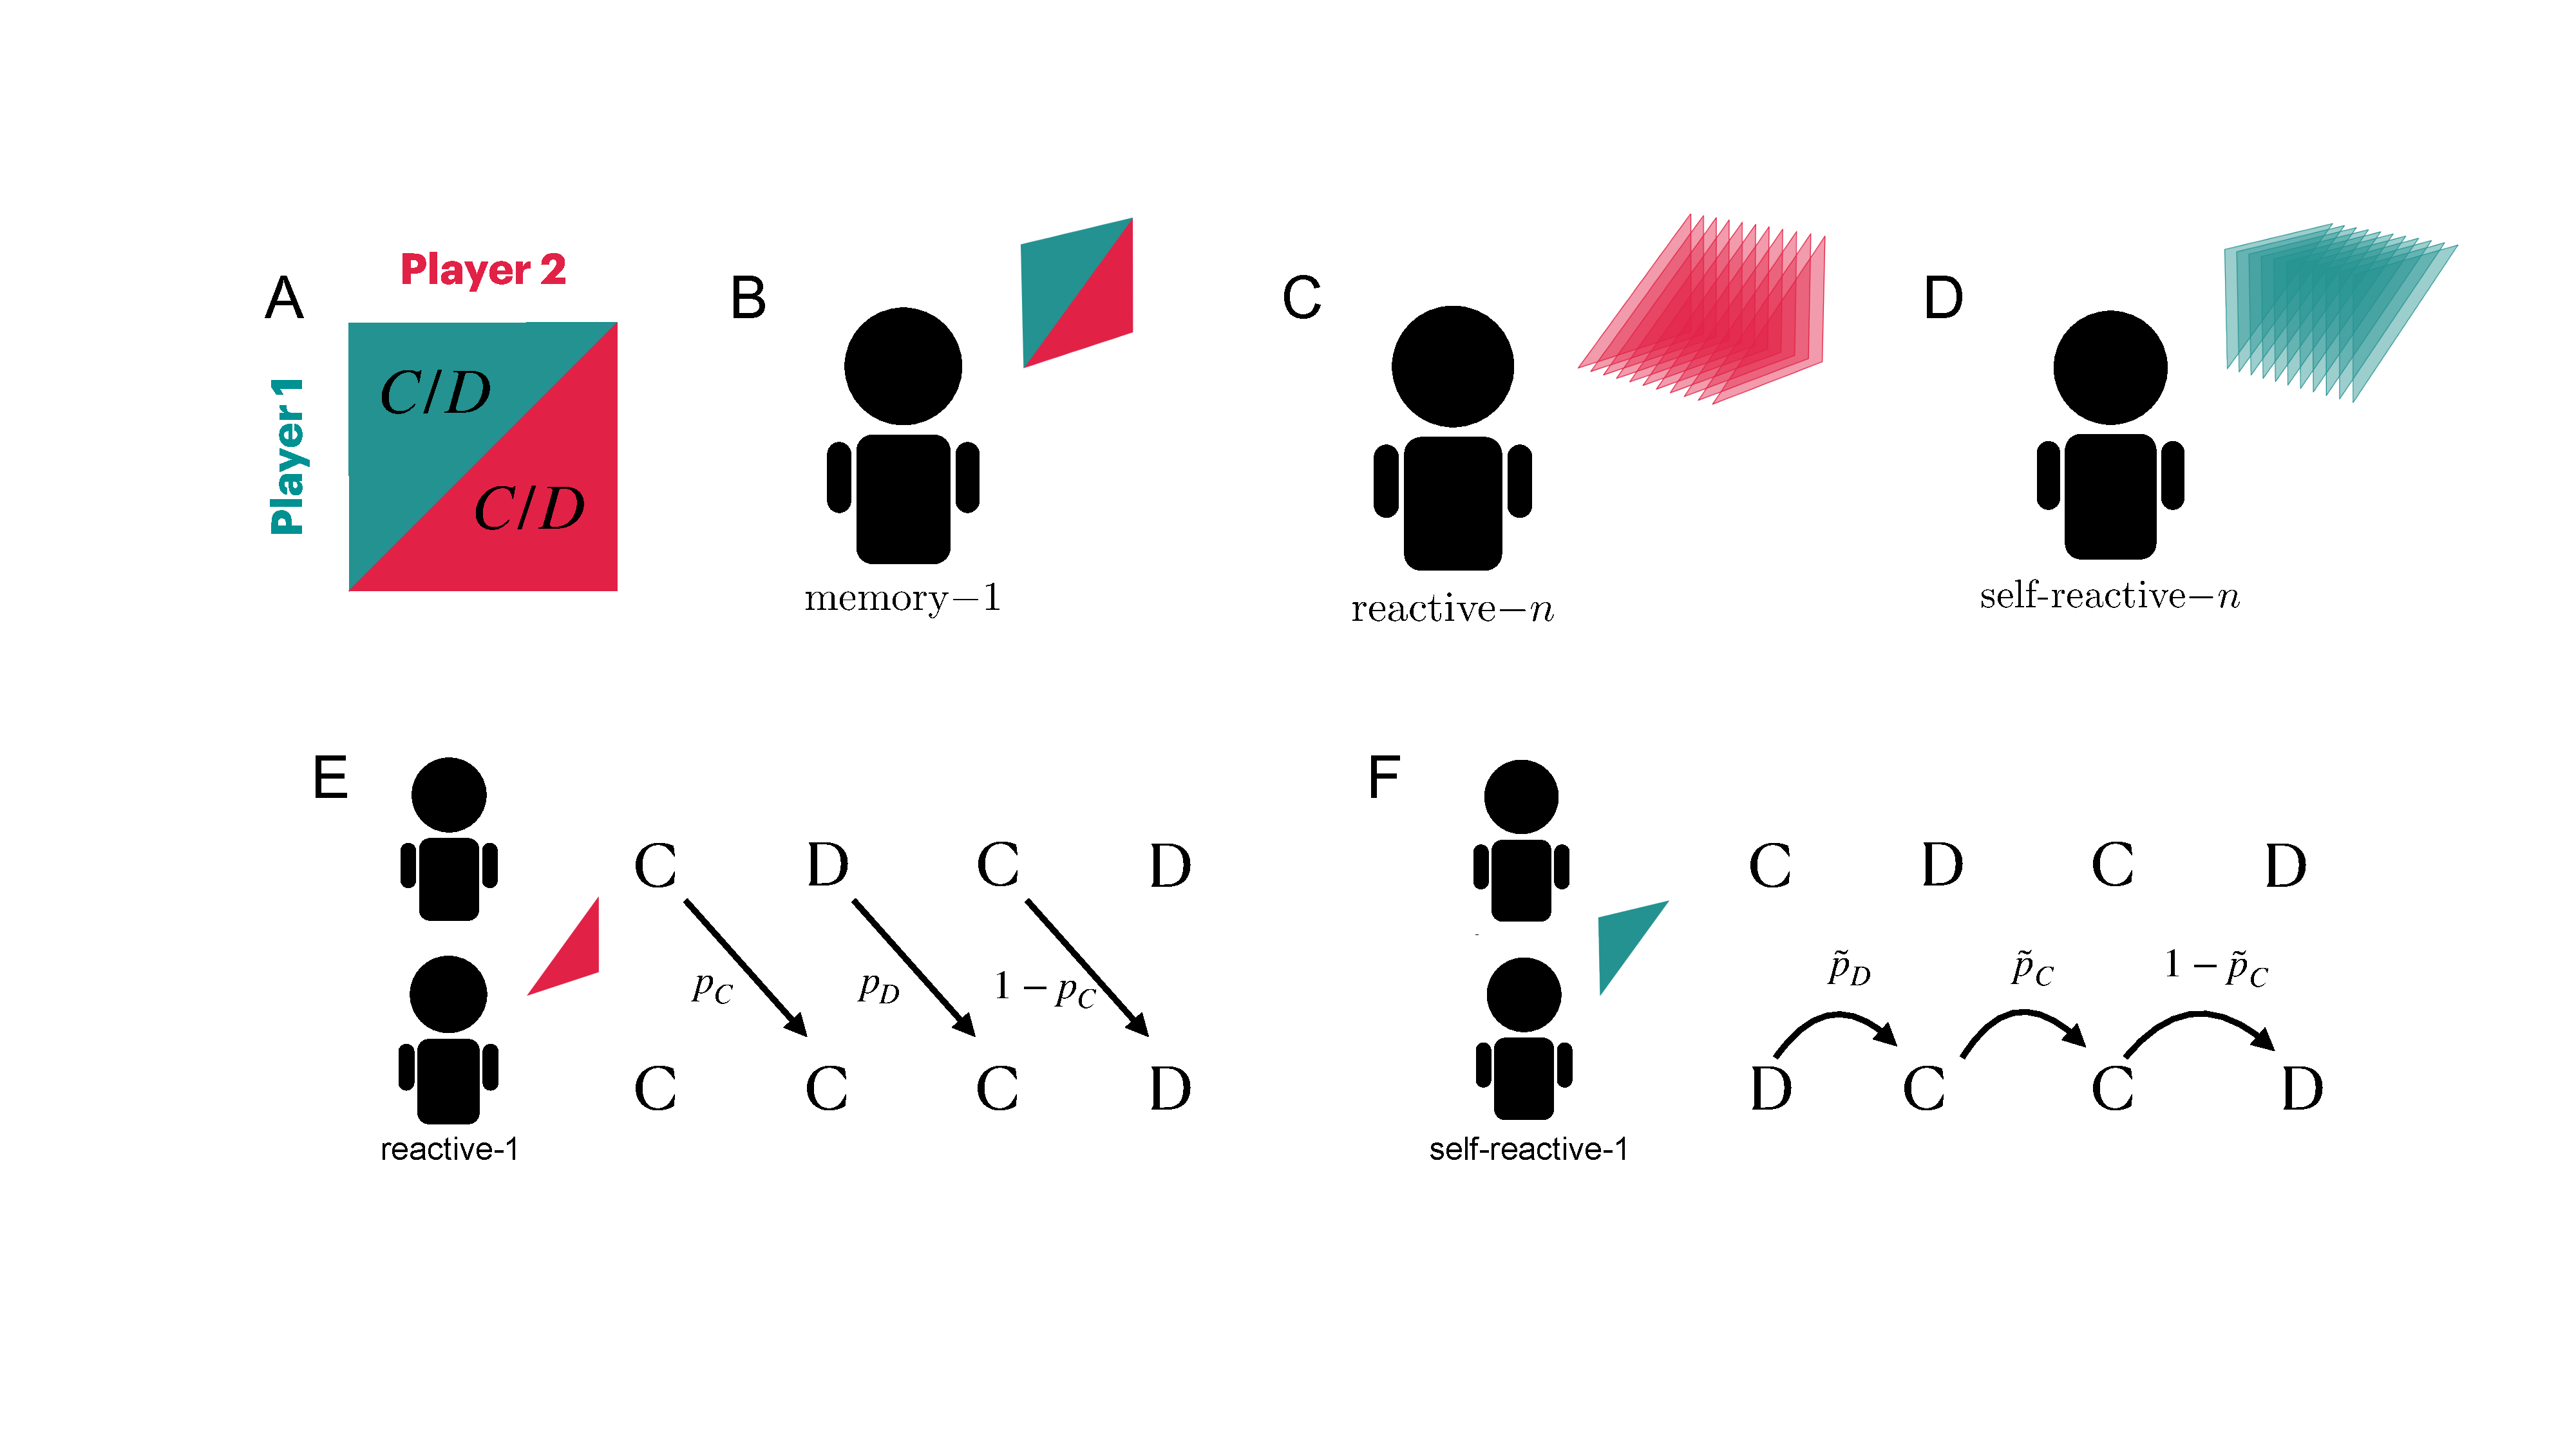
\includegraphics[width=.75\textwidth]{figures/conceptual_figure_model.pdf}
    \caption{\textbf{Model.} \textbf{A.} At each turn $t$ of the repeated game,
    players \(p\) and \(q\) decide on an action \(a^{p}_{t}, a^{q}_{t} \in \{C,
    D\}\), respectively. \textbf{B.} Memory$-1$ strategies are a set of very well
    studied strategies that use the actions of both player at round $t-1$ to
    decide on round $t$. In the graphical representation of memory-$1$ strategy
    we demonstrate this by using a single full shaded square. \textbf{C.} In this work we
    focus on reactive strategies, strategies that consider only the
    co-players actions $h^q$. This is demonstrated in the graphical representation
    by the shaded bottom half of the squares. \textbf{E.} Let the case of $n=1$, a $1-$bit
    reactive strategy is a vector $\mathbf{\hat{p}}=(\hat{p}_{C}, \hat{p}_{D})$. $\hat{p}_C$
    is the probability of cooperating given that the co-player cooperated and $\hat{p}_D$
    given that they defected. Consider a 
    match between two $1-$bit reactive strategies as shown in panel \textbf{E}. The top
    player (player $\hat{p}$) cooperates with a probability $\hat{p}_C$ in the
    second round since the co-player cooperated in the first round, player
    $\hat{p}$ cooperates with a probability $\hat{p}_D$ in the second round
    since the co-player cooperated. The player defects in round 3 with a probability $1 -
    \hat{p}_C$ given that the co-player cooperated. \textbf{D.} Another strategies set that
    we consider is that of $n-$bit self reactive strategies. These are strategies that
    consider only their own previous $n$ action.}
\end{figure}

We say $\!h^q\!=\!(C,\ldots,C)$ is the full cooperation history. An $n-$bit
reactive strategy $\mathbf{\hat{p}}$ is called {\it agreeable} if it prescribes to
cooperate with probability 1 after the full cooperation history.

The strategy $\mathbf{p}$ is called a {\it partner strategy} if it is agreeable
and if expected payoffs satisfy

\begin{equation} \label{Eq:partner}
    s_{\mathbf{q}} \geq b\!-\!c \qquad \Rightarrow \qquad s_{\mathbf{q}} = s_{\mathbf{p}} =  b\!-\!c,
\end{equation}

Thus, if a player uses a partner strategy, both players can share the rewards
fairly. However, if a co-player prefers an unfair approach, they will receive a
reduced payoff as a consequence. Partner strategies, by definition, are best
responses to themselves, making them Nash equilibria~\cite{Hilbe:GEB:2015}. We
wish to characterise all partner $n-bit$ reactive strategies of the repeated
donation game.

\section{Results}

\subsection{Sufficiency of self reactive strategies}

To characterize all partner $n$-bit reactive strategies, one would usually
need to check against all pure $n$-memory one strategies~\cite{mcavoy:PRSA:2019}.
However, we demonstrate that when player $p$ employs an $n$-bit reactive strategy,
it is sufficient to check only against $n-$bit self-reactive strategies. This
finding aligns with the previous result by Press and Dyson~\cite{press:PNAS:2012}.

More specifically, the result states that for any memory-n strategy used by
player $q$, player $p$s' score is exactly the same as if $q$ had played a
specific self-reactive memory-$n$ strategy.

A ``maybe'' example will consider the reactive $\mathbf{\hat{p}} = (0, 1)$ and the
memory-1 strategy Pavlov or Win Stay Lose Shift $\mathbf{p} = (1, 0, 0, 1)$.

\subsection{$2-$bit partner strategies}

For $n=2$, $\mathbf{\hat{p}}=(\hat{p}_{CC}, \hat{p}_{CD}, \hat{p}_{DC}, \hat{p}_{DD})$, where
$\hat{p}_{CC}$ is the probability of cooperating in round \(t\) when the
co-player cooperated in the last 2 rounds, $\hat{p}_{CD}$ is the probability of
cooperating given that the co-player cooperated in the second to last round and
defected in the last, and so on. An agreeable 2-bit strategy is represented by
the vector $\mathbf{\hat{p}}=(1, \hat{p}_{CD}, \hat{p}_{DC}, \hat{p}_{DD})$:

An agreeable $2-$bit reactive strategy is a partner strategy if the entries of
$\mathbf{\hat{p}}$ satisfy:

\begin{equation}\label{eq:two_bit_conditions}
  \displaystyle \hat{p}_{DD} < 1\!-\! \frac{c}{b}  ~~and~~ \displaystyle \frac{\hat{p}_{CD} + \hat{p}_{DC}}{2} < 1- \frac{1}{2} \cdot \frac{c}{b}.
\end{equation}

A special case of $2-$bit reactive strategies is the {\it $2-$bit counting
reactive} strategies. These are strategies that respond to the action of the
co-player, but they do not differentiate between when defection occurs, only if
one or two defections occurred. Let \(r_i\) be the probability of cooperating
given that the co-player cooperated \(i\) number of times in the last 2 turns.

Thus, $r_2 = \hat{p}_1, r_1 = \hat{p}_2 =  \hat{p}_3, r_0 = \hat{p}_4$ and
$\mathbf{\hat{p}}=(r_2=1, r_1, r_0)$. Conditions~(\ref{eq:two_bit_conditions})
then become:

\begin{equation}\label{eq:counting_two_bit_conditions}
  \displaystyle r_1 < 1-\frac{1}{2} \cdot \frac{c}{b} ~~and~~ r_0 < 1\!-\! \frac{c}{b}.
\end{equation}

\subsection{$3-$bit partner strategies}

For $n=3$, $\mathbf{\hat{p}}=(\hat{p}_{CCC}, \hat{p}_{CCD}, \hat{p}_{CDC},
\hat{p}_{CDD}, \hat{p}_{DCC}, \hat{p}_{DCD}, \hat{p}_{DDC}, \hat{p}_{DDD})$
where $\hat{p}_{CCC}$ is the probability of cooperating in round $t$ when the
co-player cooperates in the last 3 rounds, $\hat{p}_{CCD}$ is the probability of
cooperating given that the co-player cooperated in the third and second to last
rounds and defected in the last, etc. An agreeable $3-$bit strategy is of the
vector $\mathbf{\hat{p}}=(1, \hat{p}_{CCD}, \hat{p}_{CDC}, \hat{p}_{CDD},
\hat{p}_{DCC}, \hat{p}_{DCD}, \hat{p}_{DDC}, \hat{p}_{DDD})$.

An agreeable $3-$bit reactive strategy is a partner strategy if the entries of
$\mathbf{\hat{p}}$ satisfy:

\begin{align}\label{eq:three_bit_conditions}
  \frac{\hat{p}_{CCD} + \hat{p}_{CDC} + \hat{p}_{DCC}}{3} < 1\!-\! \frac{1}{3} \cdot \frac{c}{b} & \qquad 
  \frac{\hat{p}_{CDD} + \hat{p}_{DCD} + \hat{p}_{DDC}}{3} < 1\!-\! \frac{2}{3} \cdot \frac{c}{b} & \qquad 
  \hat{p}_{DDD} < 1\!-\! \frac{c}{b} \\
  & \frac{\hat{p}_{CCD} + \hat{p}_{CDD} + \hat{p}_{DCC} + \hat{p}_{DDC}}{4}  < 1\!-\! \frac{1}{2} \cdot \frac{c}{b} 
  & \qquad \frac{\hat{p}_{CDC} + \hat{p}_{DCD}}{2} < 1\!-\! \frac{1}{2} \cdot \frac{c}{b}
\end{align}

A special case of $3-$bit reactive strategies are the $3-$bit counting reactive
strategies. Let $r_i$ be the probability of cooperating given that the co-player
cooperated $i$ number of times in the last 3 turns. So, $r_3 = \hat{p}_{CCC},
r_2 = \hat{p}_{CCD} =  \hat{p}_{CDC} = \hat{p}_{DCC}, r_1 = \hat{p}_{CDD} =
\hat{p}_{DCD} =  \hat{p}_{DDC}, r_0 = \hat{p}_{CCC}$ and $\mathbf{\hat{p}}=(r_3=1,
r_2, r_1, r_0)$. Then, conditions~(\ref{eq:three_bit_conditions}), the
conditions for being a partner strategy become:

\begin{equation}\label{eq:counting_three_bit_conditions}
  \displaystyle r_2 < 1- \frac{1}{3} \cdot \frac{c}{b}, \quad r_1 < 1- \frac{2}{3} \cdot \frac{c}{b} ~~and~~ r_0 < 1\!-\! \frac{c}{b}.
\end{equation}


\subsection{$n-$bit counting partner strategies}

In the case of counting reactive strategies, we observe a pattern in the
conditions they must satisfy to be partner strategies. We show that for an $n-$bit
counting reactive strategy to be a partner strategy, the strategy's entries must
satisfy the conditions:

\begin{align*}
    r_{n}   = & 1 \\
    r_{n-1} \leq & 1  - \frac{(n - 1)}{n} \times \frac{c}{b}\\
    r_{n-2} \leq & 1  - \frac{(n - 2)}{n} \times \frac{c}{b}\\
    & \vdots \\
    r_{0} \leq &  1  - \frac{c}{b}\\
\end{align*}

\subsection{Evolutionary Dynamics}

\begin{figure}[h!]
  \centering
  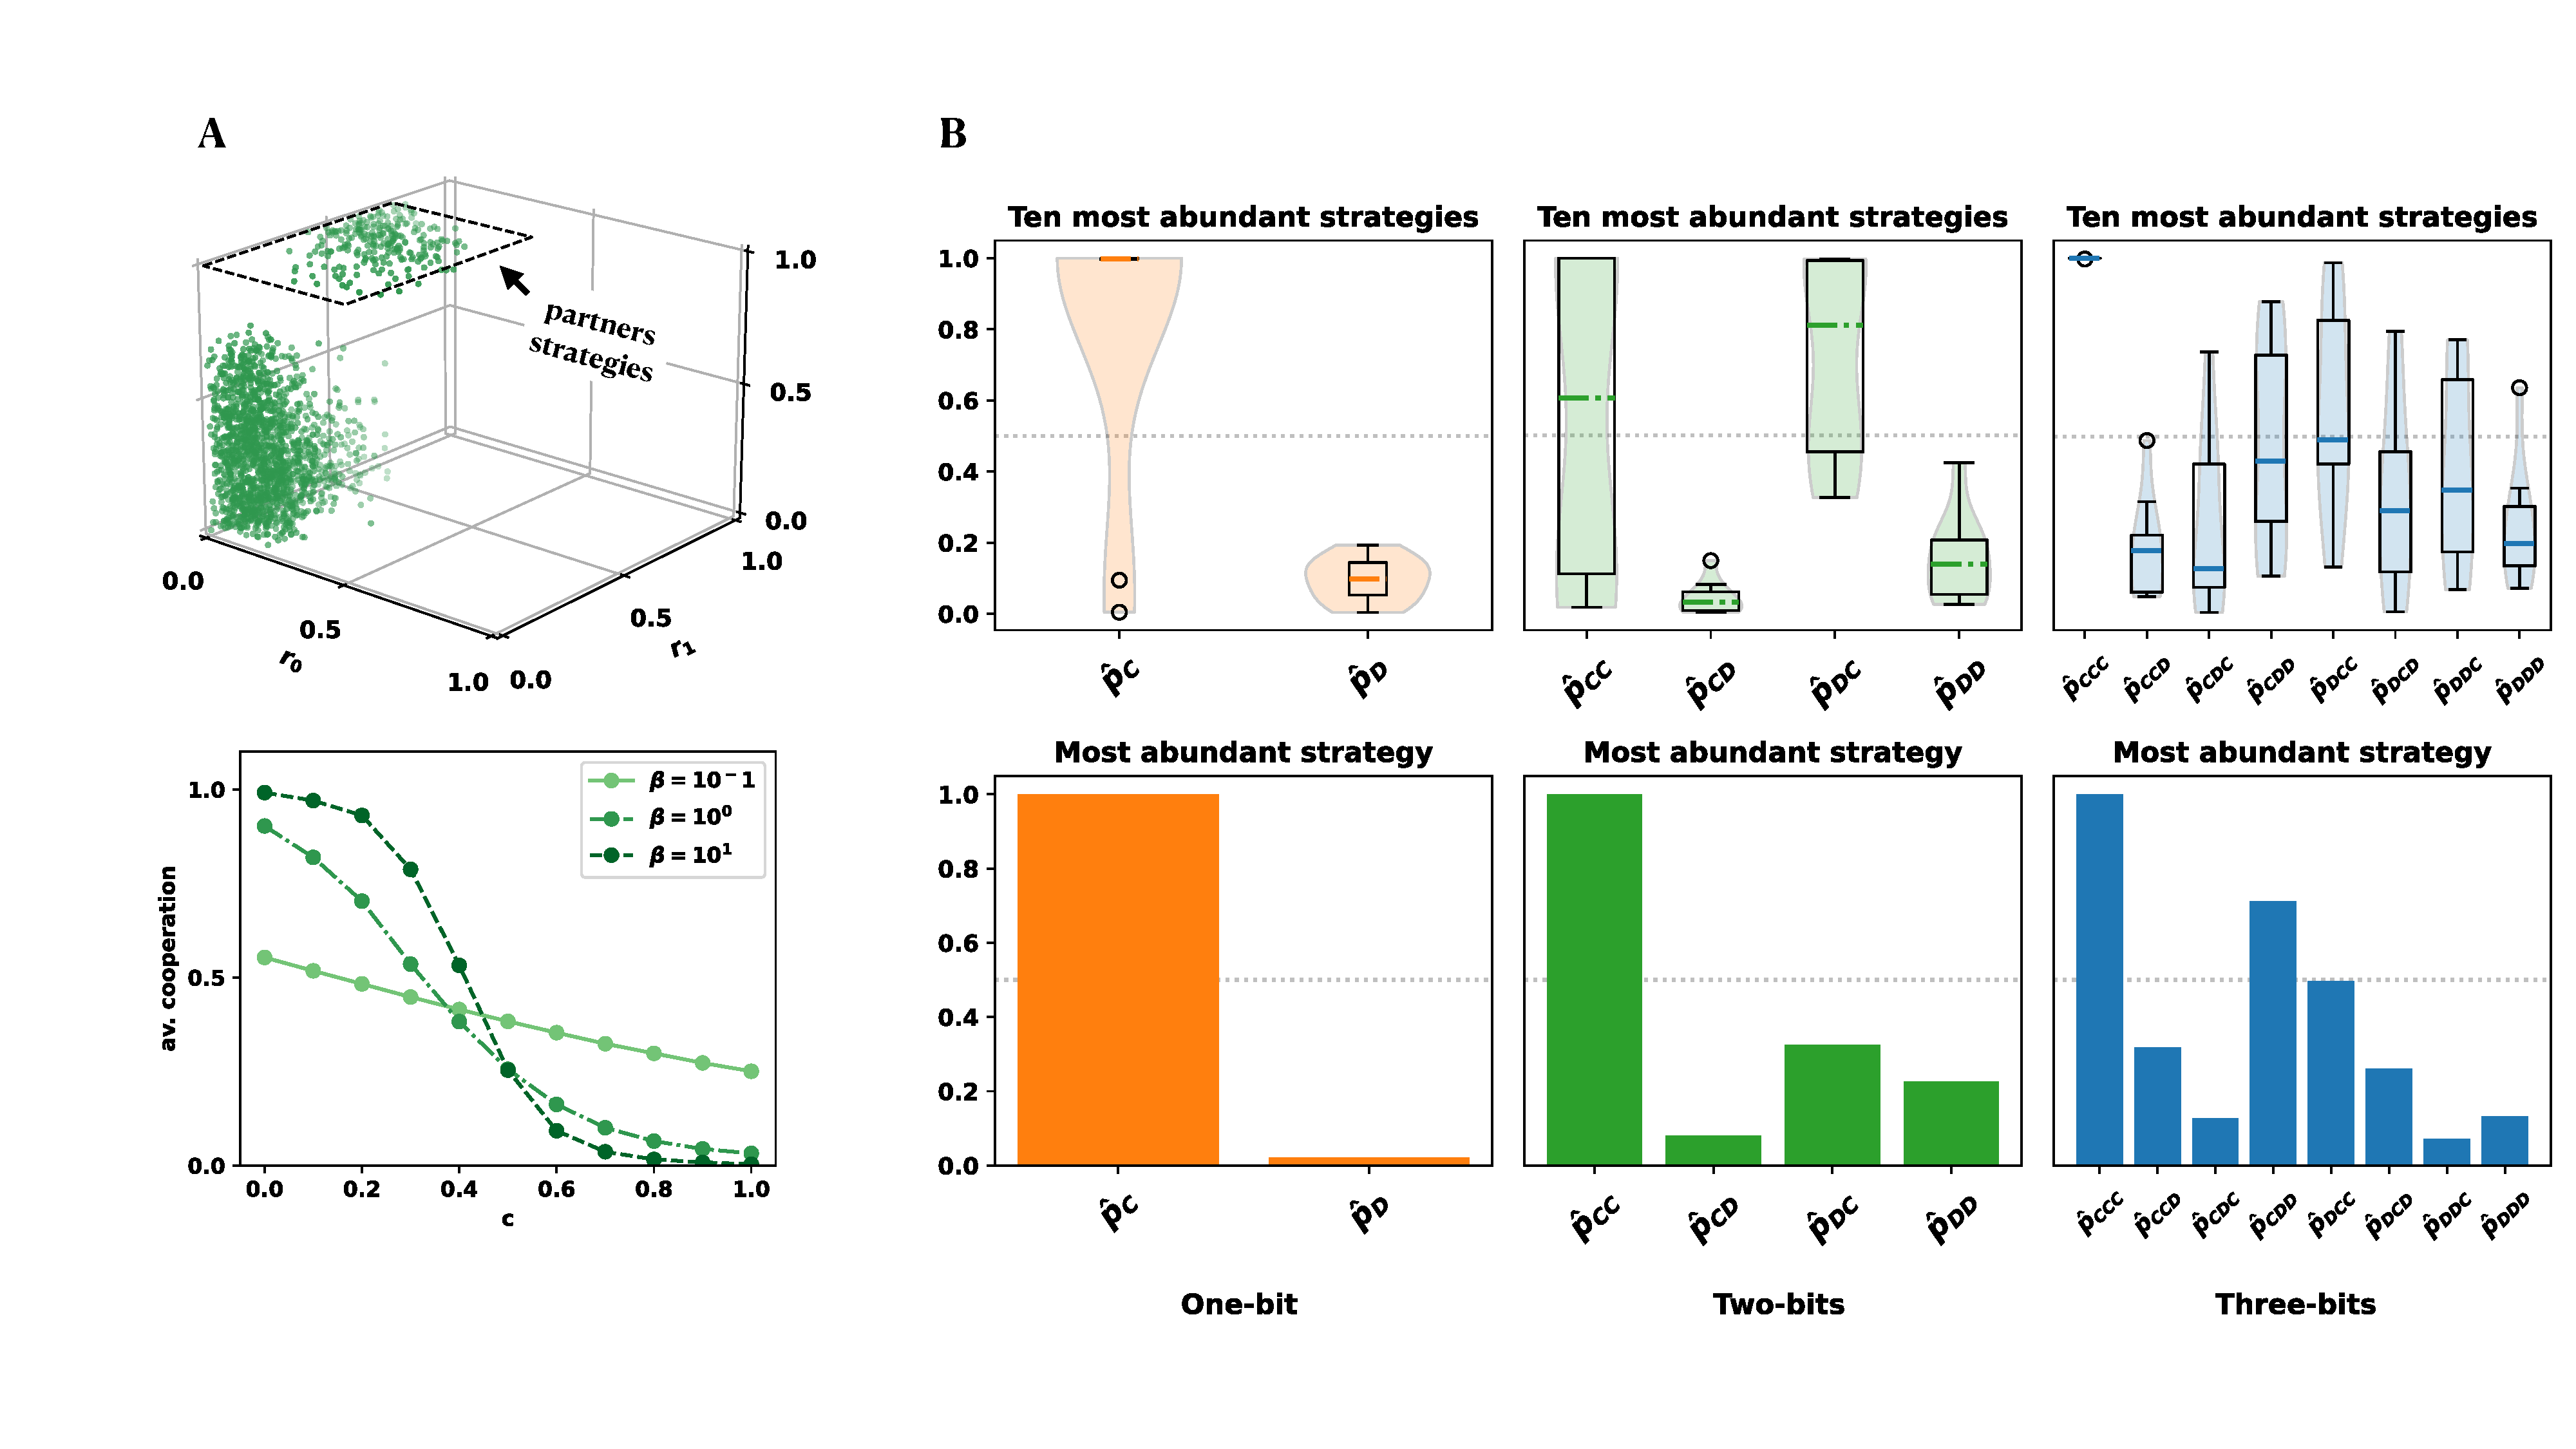
\includegraphics[width=\textwidth]{figures/evolutionary_dynamics_one_two_three.pdf}
  \caption{\textbf{Evolving strategies for $n=1, n=2$ and $n=3$.} In the previous sections we have
  characterized partners strategies for two and three bit reactive cases, and we
  have also discussed the case of counting reactive strategies. Here we want to
  assess whether partner strategies are strategies that evolve, thus are beneficial to
  adopt in an evolutionary setting. We ran simulations based on Imhof and Nowak.
  For a single run of the evolutionary process, we record the cooperating
  probabilities of the resident at each elementary time step. \textbf{A. Counting
  two-bit reactive strategies}. In the top panel we show the most abundant
  strategies of the evolutionary process when the population can use any
  counting two-bit reactive strategy ($r_0, r_1, r_2$). The abundant
  strategies are the residents that were fixed for the most time steps.
  The most abundant strategies fall within the region of the partner strategies.
  In the bottom panel we look at the evolving cooperation rate closer. The
  average cooperation is calculated by considering the cooperation rate within
  the resident population. For a given $\beta$ value we vary the cost $c \in [0, 1]$
  whilst we have fixed $b=1$. Three curves are shown, these are for different values
  of selection strength, $\beta \in {10^-1, 10^0, 10^1}$.
  \textbf{B. One, two, three bits.} We ran 10 independent simulations for each
  set of strategies and recorded the most abundant strategy for each run. The
  abundant strategy is the resident that was fixed for the most time steps. For
  the simulations we used \(b=1 \text{ and } c=.5\). For $n$ equal to 1 and
  2, \(T= 10 ^ 7\) and for $n=3$ then \(T= 2 \times10 ^ 7\).}
\end{figure}

\begin{figure}[h!]
  \centering
  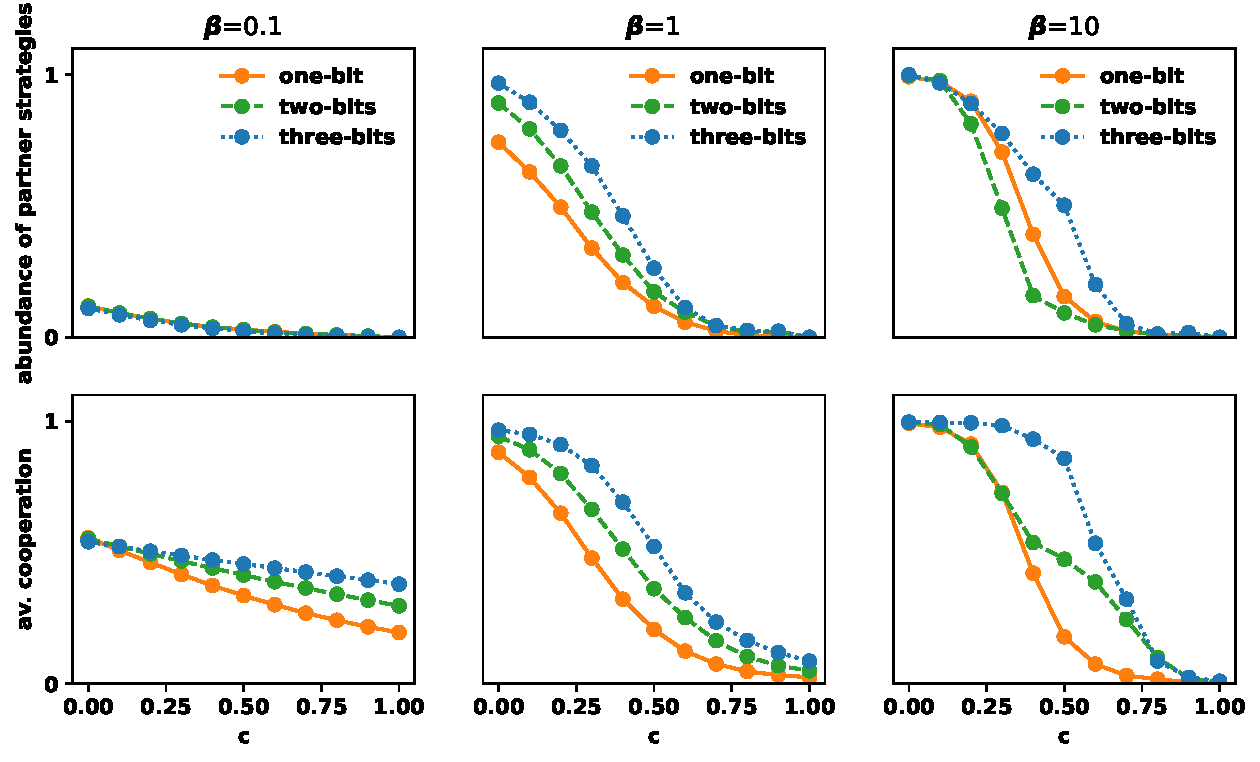
\includegraphics[width=\textwidth]{figures/abundance_of_partner_strategies.pdf}
  \caption{\textbf{Abundance of partner strategies.}
  We ran simulations based on Imhof and Nowak, varying the cost ($c$) and
  strength of selection ($\beta$). The cooperation benefit ($b$) is fixed at a
  value of 1. The results demonstrate that partner strategies evolve notably
  under strong selection ($\beta=1$) and lower cost conditions. Furthermore, the abundance
  of partner strategies is consistently higher when individuals have access to
  greater memory. The bottom panel displays how these partner strategies lead to
  increased levels of cooperation.}
\end{figure}

\section{Discussion}

~\\
\bibliography{bibliography.bib}

\end{document}